\section{Results and Discussion}\label{sec:results}

\subsection{Experimental Setup}\label{sec:setup}
The questionnaire has not been administered yet, so this draft contains no
estimates of teacher burnout; the measurements below concern only the
pipeline. They were made on ``synthetic respondents'' with the MBI structure,
on one machine inside one Docker image (Python 3.11.9), with seed 42. Ten
warm-up runs were discarded, then 40 measured runs were recorded for each
workload, interleaved in turn. Outliers (\autoref{eq:iqr}) were flagged but kept. The baseline is the
smallest workload, $n_0=35$, which equals the planned sample size
(\autoref{tab:params}). Six edge-case scenarios were also run five times each.

\subsection{Results}\label{sec:res}
\autoref{tab:results} and \autoref{fig:results} summarise the 120 measured
runs. All of them finished without an error (error rate 0\,\%), and nine runs
were flagged as outliers (3, 4 and 2 for $n=35$, 100 and 1000). The mean latency
for $n=35$ and $n=100$ (45.1 and 44.8\,ms) is higher than the median, which
indicates right-skewed run times; therefore medians and percentiles are reported. Re-running the aggregation with the
same seed gave identical statistics, which is the reproducibility check of the pipeline. \autoref{tab:edge} shows the edge cases: four invalid
inputs were rejected with an explicit message instead of being scored silently,
while two scenarios were processed. The median latency was
43.9\,ms for $n=35$, 43.8\,ms for $n=100$ and 46.8\,ms for $n=1000$. The
throughput grew almost in proportion to the workload: $S(100)=2.86$ and
$S(1000)=26.8$, that is, $E(100)=1.00$ and $E(1000)=0.94$ (\autoref{eq:speedup}).

\begin{table}[b]
  \centering
  \caption{Comparison of the workloads with the baseline $n_0=35$ (40 runs
  each). Median latency with its 95\,\% bootstrap interval; p95 and p99 in ms;
  throughput in respondents per second; speed-up $S(n)$ from \autoref{eq:speedup}.}
  \label{tab:results}
  \footnotesize
  \setlength{\tabcolsep}{3pt}
  \begin{tabular}{@{}rcccrr@{}}
    \toprule
    $n$ & Median (ms) & p95 & p99 & Resp./s & $S(n)$ \\
    \midrule
    35 (baseline) & 43.9 [43.0, 44.6] & 53.8 & 64.1 & 797 & 1.00 \\
    100  & 43.8 [43.0, 45.1] & 53.3 & 59.0 & 2\,283 & 2.86 \\
    1000 & 46.8 [46.2, 47.9] & 55.3 & 82.1 & 21\,371 & 26.8 \\
    \bottomrule
  \end{tabular}
\end{table}

\begin{table}[b]
  \centering
  \caption{Edge-case scenarios (five runs each) and the behaviour of the pipeline.}
  \label{tab:edge}
  \footnotesize
  \begin{tabular}{@{}llc@{}}
    \toprule
    Scenario & Input & Outcome \\
    \midrule
    Missing values & empty item answers & rejected \\
    Out of range & answers outside 0--6 & rejected \\
    Single group & only one school type & rejected \\
    Duplicates & repeated respondent IDs & rejected \\
    Tiny groups & very small groups & processed \\
    Straight-lining & identical answers to all items & processed \\
    \bottomrule
  \end{tabular}
\end{table}

\begin{figure*}[t]
  \centering
  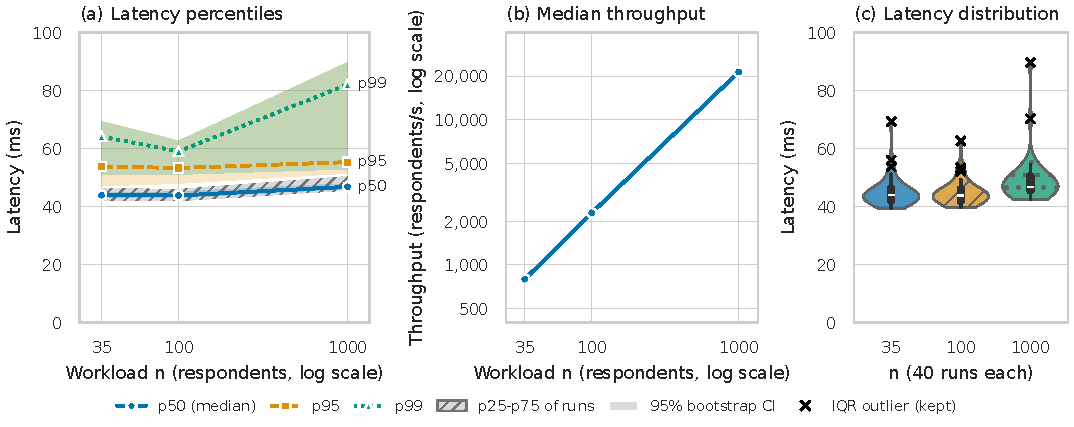
\includegraphics[width=\textwidth]{fig_combined_latency_throughput.pdf}
  \caption{Latency and throughput for $n=35$, 100 and 1000 synthetic respondents
  (40 runs each). (a)~Latency percentiles; bands are 95\,\% bootstrap intervals
  ($B=10\,000$), the hatched band is the interquartile range of the runs.
  (b)~Median throughput on logarithmic axes. (c)~Distribution of the run
  latencies; crosses mark outliers (9 of 120), which were kept.}
  \label{fig:results}
\end{figure*}

\subsection{Discussion}\label{sec:disc}
The median latency rose by only about 3\,ms (roughly 7\,\%) while the workload
grew 28-fold. This suggests that the time of a run is dominated by a fixed
overhead and not by the number of respondents. Relative to the baseline, the
larger workloads therefore cost little extra time, and since the planned sample
is of the baseline size, re-running the analysis after every data update appears
practical (the third and fourth contributions in \autoref{sec:intro}). At the measured median, a thousand repetitions of the full analysis on
1000 respondents would take roughly 47 seconds. The intervals
of the medians for $n=35$ and $n=100$ overlap, so the data do not distinguish
them, while the interval for $n=1000$ does not overlap either of them.

Tail percentiles matter for responsiveness~\cite{dean2013tail}, but here they are
the least certain values: with 40 runs, the 99th percentile is determined by the
one or two slowest runs. Its rise at $n=1000$ (82.1\,ms) is therefore a hint, not
an established effect. The analysis plan is fixed in advance (\autoref{tab:plan}), which limits the room for
analytic choices after the data have been seen. Finally, the review of teacher burnout reports that prevalence
depends on the instrument~\cite{garciacarmona2019burnout}; within the scope of our
design, this supports analysing all respondents with one instrument and one fixed protocol
(\autoref{sec:method}). Rejecting invalid input (\autoref{tab:edge}) protects later conclusions from
silent scoring errors. The measurements say nothing about burnout itself---they describe the software only.
